%#Split: 02_purpose_plan  
%#PieceName: p02_purpose_plan
% p02_purpose_plan_00.tex
\KLBeginSubjectWithHeaderCommands{02}{}{研究目的・内容等}{2}{F}{}{\DCPDFirstSubjectPageStyle}{\DCPDDefaultPageStyle}

\section{研究目的・内容等}
%    <<最大 2ページ>>

%s02_purpose_plan_dcpd
%begin 研究目的と研究計画short留意事項なし ====================
\noindent[\textcircled{1}\textbf{研究目的}]
% 速度
% セキュリティ(検証)
% 利便性

本研究の理想は\amikake{\textbf{「クラウドベンダ」への信用を「クラウドコンピューティング」から取り除く}}ことである。そのための一歩として本研究では、\ref{aim:linearmk}線形計算量3パーティ拡張を\ref{aim:exec}暗号上プログラム実行基盤として利便性を保ちながら行い、\ref{aim:verify}計算結果の検証も可能とし、AWSなどのパブリッククラウドで動作するプロトタイプ実装も開発する。図\ref{fig:solution}にこれらを統合した本研究で提案するプロトコルを示す。

% ロックと鍵を小さく
\begin{figure}[h]
    \centering
    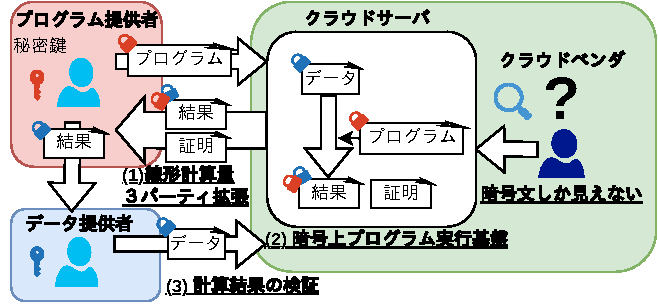
\includegraphics[width=0.8\linewidth]{figures/solution.drawio.pdf}
    \vspace*{-0.5cm}
    \caption{本研究の提案するプロトコル}
    \label{fig:solution}
\end{figure}

\noindent [\textcircled{1}\textcircled{2}\textbf{研究内容・研究方法・どこまで明らかにするか}]
% (2)は衝突するので修正

\begin{enumerate}[label=(\Roman*),leftmargin=1cm]
\setlength{\parskip}{0cm} % 段落間
\setlength{\itemsep}{0cm} % 項目間
\item \underline{\textbf{線形計算量3パーティ拡張}}: MK-TFHE(Multi Key TFHE)~\ref{paper:mktfhe}は3パーティ環境において、\ref{prob:maliciousvender}データとプログラムがクラウドベンダに見えることを防げる。しかし、計算量が鍵の本数の2乗に比例する欠点がある。本項目では全パーティの鍵の総和を鍵として利用するアイデア~\ref{paper:keylift}をMK-TFHEに適用することで、\amikake{\textbf{計算量を鍵の本数に線形に比例}}させる方法を明らかにする。\label{aim:linearmk}

\item \underline{\textbf{暗号上プログラム実行基盤}}: 
準同型暗号上の計算は特有の表現を使う必要があり、通常のプログラムそのままでは実行できない。\ref{prob:usability}利便性が損なわれることを防ぐため、本項目ではRISC-V CPUの\amikake{\textbf{論理回路を暗号上で実行}}することで、プログラムをそのまま実行する方法を明らかにする。さらに、\ref{aim:linearmk}による速度低下を並列化で補う手法、\ref{aim:verify}が行いやすくなるCPUの設計法も明らかにする。\label{aim:exec}

\item  \underline{\textbf{計算結果の検証}}: \ref{prob:verifiability}実行結果がプログラムの出力だと保証できないことは\amikake{\textbf{準同型暗号にVCを統合}} することで解決できる。そのような手法には、(a)準同型暗号の実行自体を検証する方法~\ref{paper:boostVC}と、(b)準同型暗号上の計算を検証する方法~\ref{paper:nivc}の2種類がある。本項目では\ref{aim:linearmk}と\ref{aim:exec}と統合する上で(a),(b)のどちらがセキュリティ的・性能的に優れているかを明らかにする。\label{aim:verify}
\end{enumerate}

\noindent[\textcircled{\scriptsize 2}\textbf{研究計画}]

\noindent(申請時点から採用までの準備)
% MICROの内容は計画にする

採用までの間には\ref{aim:exec}暗号上プログラム実行基盤の実装に向け、CPU・GPU向け準同型暗号ライブラリの高速化と、準同型暗号の並列実行のためのジョブディスパッチャの複数マシンへの拡張を行う。この成果は論理回路の準同型暗号上での高速な実行基盤として国際会議に投稿予定である。

\noindent(1年目: \ref{aim:linearmk}形計算量3パーティ拡張)

採用前から改善する準同型暗号ライブラリにマルチパーティ拡張の知見~\ref{paper:keylift}を統合し、理論・実装的に高速化する。この成果はマルチパーティでの論理回路向け準同型暗号の理論・実装的改善として国際会議に投稿する。

\noindent(2年目: \ref{aim:exec}暗号上プログラム実行基盤の実装)

採用前と1年目の成果に加え、準同型暗号特有の制約を考慮した最適なCPUの設計法を開発することで、既存プログラムの暗号上での高速な実行を実現し、国際会議に投稿する。

\noindent(3年目:\ref{aim:exec}及び\ref{aim:verify}計算結果の検証)

ここまでの成果にVCの知見を統合し、準同型暗号上でのプログラム実行を検証可能にする。この成果は検証可能かつ3パーティでの既存プログラムの暗号上実行手法として国際会議に投稿する。

\begin{figure}[h]
    \centering
    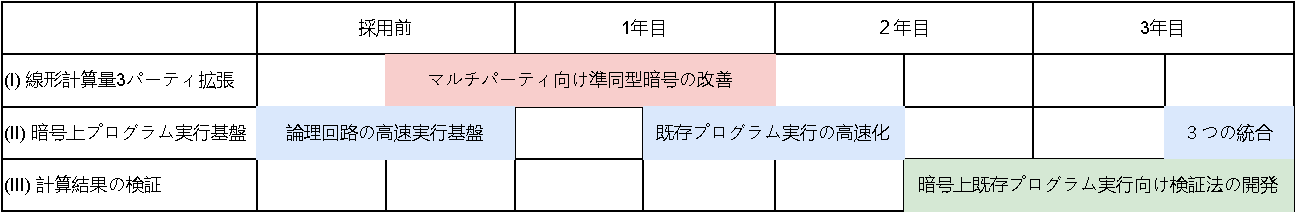
\includegraphics[width=\linewidth]{figures/schedule.drawio.pdf}
    \vspace*{-1cm}
    \caption{研究計画のタイムライン}
    \label{fig:schedule}
\end{figure}

\noindent[\textcircled{3} \textbf{特色・独創的な点}]

本研究は準同型暗号上でRISC-V CPUの論理回路を評価することで、既存プログラムの暗号上での実行を可能としつつ、3パーティかつ計算結果が検証可能という高いセキュリティを達成することが独創的な点である。特色ある点は本研究では準同型暗号ライブラリ、計算の検証、準同型暗号並列実行のためのジョブディスパッチャ、準同型暗号上で実行するRISC-V CPUをプラットフォームとして実装する点である。

\noindent[\textcircled{3}先行研究との比較]
\begin{enumerate}[label=(\Roman*),leftmargin=1cm]
\setlength{\parskip}{0cm} % 段落間
\setlength{\itemsep}{0cm} % 項目間
\item	3パーティに対応した論理回路実行に適した既存の暗号がMK-TFHE\ref{paper:mktfhe}であるが、計算量が鍵の本数の2乗に比例する欠点がある。本研究では論理回路実行に適した計算量が鍵の本数に線形に比例する準同型暗号を開発する。

\item	我々の過去の研究\ref{paper:vsp}では2パーティに限られ、計算の検証は行えていなかった。また、独自ISAのため、C言語のみのサポートにとどまっていた。本研究ではRISC-V ISAを採用することでより多くの言語を容易にサポートできるようにする。また、\ref{aim:linearmk}と\ref{aim:verify}による影響も考慮に入れた最適なCPUの設計法を明らかにする最初の研究である。

\item	準同型暗号と計算の検証を同時に行う研究は、MK-TFHE~\ref{paper:mktfhe}に適応できていないか、実装がない~\ref{paper:boostVC}。本研究は既存プログラムの暗号上での実行に適した検証法を検討し、実装を与える最初の研究である。
\end{enumerate}

\noindent[\textcircled{3} \textbf{本研究が完成したとき予想されるインパクト及び将来の見通し}]

 本研究完成の暁には、クラウドベンダへの信用を要しない選択肢が用意されることで、社会活動における特定の大企業への依存が低減されると考えている。将来の見通しとしてはクラウドコンピューティングから信用を取り除くことで、個人情報のような機微な情報を扱う場合でも\amikake{\textbf{安全に計算資源をシェア}}できるプラットフォームの構築につながると考えている。

\noindent[\textcircled{4} \textbf{申請者が担当する部分}]

本研究計画の内容はすべて申請者が担当する。

% 自分のものメインでいいかも
% 2.でまとめる
{\footnotesize
\noindent[\textbf{参考文献}]  
\begin{enumerate*}[label={[\arabic*]},leftmargin=0.5cm]
    \paper{Multi Key Homomorphic Encryption from TFHE}{H. Chen, \etal}{IACR ASIACRYPT}{}{}{2019}\label{paper:mktfhe}
    \paper{Boosting Verifiable Computation on Encrypted Data}{D Fiore, \etal}{IACR Cryptology ePrint Archive}{}{}{2020}\label{paper:boostVC}
    \paper{Non interactive verifiable computing: Outsourcing computation to untrusted workers}{R. Gennaro, \etal}{IACR CRYPTO}{}{}{2010}\label{paper:nivc}
    \paper{Virtual Secure Platform: A {Five-Stage} Pipeline Processor over {TFHE}}{Kotaro Matsuoka, \etal}{30th USENIX Security Symposium (USENIX Security 21)}{}{pp.4007--4024}{2021}\label{paper:vsp}
    % \paper{Asymptotically Faster Multi-Key Homomorphic Encryption from Homomorphic Gadget Decomposition}{T. Kim, \etal}{IACR Cryptology ePrint Archive}{}{}{2022}\label{paper:mkgd}
    \paper{Key lifting : Multi-key Fully Homomorphic Encryption in plain model}{X. Dai, \etal}{IACR Cryptology ePrint Archive}{}{}{2022}\label{paper:keylift}
\end{enumerate*}
}

%end 研究目的と研究計画short留意事項なし ====================
% p02_purpose_plan_01.tex
\KLEndSubject{F}


